\documentclass[a4paper,11pt]{article}

%=========================
% Les styles
%=========================

\usepackage{style-esi/french}	% Francise LaTeX
\usepackage{style-esi/color}	% Couleurs du thème
\usepackage{style-esi/common}	% Commun à tout type de document
\usepackage{style-esi/td}
\usepackage{style-esi/licence}	% Affiche une licence dans le document
\usepackage{style-esi/exercice}
\usepackage{style-esi/listing}

\date{2018 -- 2019}
\siglecours{DEV1}
\libellecours{Laboratoires Java I}
\libelledocument{TD1 -- Netbeans}
\sigleprof{}



%% =================================
% Style pour le cours de Java
% ---------------------------------
% \java{...} ou \code{...}
% \begin{Java}...\end{Java} 
%    ou \begin{Code}...\end{Code}
% \sigle{...}
% \emph{...}
% \begin{slidetoc}...\end{slidetoc}
% =================================

% ===== Francisation
\usepackage[frenchb]{babel}
\usepackage[latin1]{inputenc}
%\usepackage[utf8]{inputenc}
\usepackage[T1]{fontenc} 
\usepackage{lmodern}

% ===== bullets pour les items
\setbeamertemplate{itemize item}[triangle]
\setbeamertemplate{itemize subitem}[square]
\setbeamertemplate{itemize subsubitem}[circle]
\setbeamercolor{itemize item}{fg=black!70}
\setbeamercolor{itemize subitem}{fg=black!70}
\setbeamercolor{itemize subsubitem}{fg=black!70}

% ===== Pour utiliser \ding
\usepackage{pifont}

% ===== Pour pouvoir barrer du texte (\sout)
\usepackage{ulem}

% ===== Emphase de texte
\mode<beamer>{ 
	\setbeamercolor{description item}{fg=brown} 
	\renewcommand{\emph}[1]{\textbf{\color{brown}{#1}}}
}
\mode<handout>{ 
	\setbeamercolor{description item}{fg=black} 
	\setbeamerfont{description item}{series=\bfseries} 
	\renewcommand{\emph}[1]{\textbf{\color{black}{#1}}}
}

% ===== Insertion de code + Java + sigle
% ----- Environnement Verbatim
% ----- Code : pour du code non java (shell, output, ...)
% ----- Java : pour du code Java
% L'argument optionnel permet d'adapter la mise en page
% ex: \begin{Java}[basicstyle=\scriptsize] pour du code plus petit
% Mettre le frame en fragile
\usepackage{listings}
\lstdefinestyle{lstverb}
  {
    backgroundcolor=\usebeamercolor[bg]{block body},
    frameround=tttt, frame=trbl, framerule=0pt,
    basicstyle=\footnotesize,
    lineskip=-1pt,   % pour rapprocher les lignes
    flexiblecolumns, 
    extendedchars=true
  }
\lstnewenvironment{Java}[1][]{\lstset{style=lstverb,language=java,#1}}{}
\lstnewenvironment{Code}[1][]{\lstset{style=lstverb,#1}}{}
\mode<beamer>{
  \newcommand{\java}{\lstinline[language=java,basicstyle=\color{blue!70!black}] 
  } %[
  \newcommand{\code}{\lstinline[basicstyle=\color{blue!70!black}] 
  } %[
}
\mode<handout>{
  \newcommand{\java}{\lstinline[language=java,basicstyle=\color{black}]
  } %[
  \newcommand{\code}{\lstinline[basicstyle=\color{black}]
  } %[
}
\newcommand{\sigle}[1]{{\ttfamily \bfseries #1}}

% ===== Pour les grammaires : \begin{grammaire}...\end{grammaire}
\usepackage{fancyvrb}
\DefineVerbatimEnvironment{grammaire}{Verbatim}%
  {frame=lines,commandchars=\\\{\},baselinestretch=0.9,%
   fontfamily=helvetica,fontsize=\footnotesize,obeytabs=true,formatcom=\color{black!80}%
   }
\newcommand{\term}[1]{{\ttfamily \bfseries #1}}
\newcommand{\oterm}[1]{{\ttfamily \bfseries #1}{\tiny (opt)}}
\newcommand{\nterm}[1]{\textit{#1}}
\newcommand{\onterm}[1]{\textit{#1}{\tiny (opt)}}
\newcommand{\opt}{{\tiny(opt)} }
\newcommand{\shaded}[1]{{\color{black!30} #1}}

% === Diff�rentes pages de garde pour les le�ons

\newcommand{\leconwithtoc}{
\begin{frame}[plain]
\begin{block}{\center S�ance \thesection}
  {
  \begin{center}
  \insertsection
  \end{center}
  \begin{multicols}{2}
  \tableofcontents[sectionstyle=hide,subsectionstyle=show/show/hide]
  \end{multicols}
  \bigskip
  }
\end{block}
\end{frame}
}

\newcommand{\leconwithtoconecol}{
\begin{frame}
\begin{block}{\center S�ance \thesection}
  {
  \begin{center}
  \insertsection
  \end{center}
  \tableofcontents[sectionstyle=hide,subsectionstyle=show/show/hide]
  \bigskip
  }
\end{block}
\end{frame}
}

\newcommand{\leconwithtocquote}[1]{
\begin{frame}
\begin{block}{\center S�ance \thesection}
  {
  \begin{center}
  \insertsection
  \end{center}
  \begin{multicols}{2}
  \tableofcontents[sectionstyle=hide,subsectionstyle=show/show/hide]
  \end{multicols}
  \bigskip
  }
\end{block}
\bigskip
  \begin{flushright}
  \small\textit{#1}
  \end{flushright}
\end{frame}
}

\newcommand{\leconwithtocinside}{
\begin{frame}
\begin{block}{\center O� en sommes-nous ?}
  {
  \par
  \bigskip
  \tableofcontents[sectionstyle=hide,subsectionstyle=show/shaded/hide]
  \bigskip
  }
\end{block}
\end{frame}
}

\newcommand{\leconwithabstract}[1]{
\begin{frame}
\begin{block}{\center Le�on \thesection\ --- \insertsection}
  {
  \medskip
  \begin{center}
  \textit{#1}
  \end{center}
  }
\end{block}
\end{frame}
}

\newcommand{\leconwithabstracttoc}[1]{
\begin{frame}
\begin{block}{\center Le�on \thesection\ --- \insertsection}
  {
  \medskip
  \textit{#1}
  \bigskip
  \tableofcontents[sectionstyle=hide,subsectionstyle=show/show/hide]
  \bigskip
  }
\end{block}
\end{frame}
}

\newcommand{\leconwithabstractquote}[2]{
\begin{frame}
\begin{block}{\center Le�on \thesection\ --- \insertsection}
  {
  \medskip
  \begin{center}
  \textit{#1}
  \end{center}
  }
\end{block}
\bigskip
  \begin{flushright}
  \small\textit{#2}
  \end{flushright}
\end{frame}
}

\definecolor{bleu}{rgb}{0.59, 0.65, 0.82}
\usepackage{multicol}

% ===== Alerte ====
\newcommand{\warning}[1]{
  \begin{tabular}{cl}
    \begin{minipage}[c]{30pt}
    \includegraphics[width=30pt]{../img/warning}
    \end{minipage}
    & 
    \begin{minipage}[c]{270pt}
    #1
    \end{minipage}
    \\
  \end{tabular}
}

% === Image en fullscreen
% Je ne trouve pas comment faire avec une seule commande qui calcule la position
\usepackage[absolute,overlay]{textpos}
\newcommand{\imgfullw}[3]
{{
	\usebackgroundtemplate{
		\includegraphics[keepaspectratio,width=\paperwidth]{#1}}
    \setbeamertemplate{navigation symbols}{}
	\setbeamercolor{background canvas}{bg=black}
	\begin{frame}[plain]{}
		#2
		\begin{textblock*}{\linewidth}(0pt,.87\paperheight)
			\tiny\flushright{\color{gray}\href{#3}{Cr�dit photo}}
		\end{textblock*}
	\end{frame}
}}

\newcommand{\imgfullwt}[3]
{{
	\usebackgroundtemplate{
		\includegraphics[keepaspectratio,width=\paperwidth]{#1}}
    \setbeamertemplate{navigation symbols}{}
	\setbeamercolor{background canvas}{bg=black}
	\begin{frame}[plain,t]{}
		#2
		\begin{textblock*}{\linewidth}(0pt,.87\paperheight)
			\tiny\flushright{\color{gray}\href{#3}{Cr�dit photo}}
		\end{textblock*}
	\end{frame}
}}

\newcommand{\imgfullh}[3]
{{
	\usebackgroundtemplate{
		\includegraphics[keepaspectratio,height=\paperheight]{#1}}
    \setbeamertemplate{navigation symbols}{}
	\setbeamercolor{background canvas}{bg=black}
	\begin{frame}[plain]{}
		#2
		\begin{textblock*}{\linewidth}(0pt,.9\paperheight)
			\tiny\flushright{\color{gray}\href{#3}{Cr�dit photo}}
		\end{textblock*}
	\end{frame}
}}

\newcommand{\imgfullht}[3]
{{
	\usebackgroundtemplate{
		\includegraphics[keepaspectratio,height=\paperheight]{#1}}
    \setbeamertemplate{navigation symbols}{}
	\setbeamercolor{background canvas}{bg=black}
	\begin{frame}[plain,t]{}
		#2
		\begin{textblock*}{\linewidth}(0pt,.9\paperheight)
			\tiny\flushright{\color{gray}\href{#3}{Cr�dit photo}}
		\end{textblock*}
	\end{frame}
}}

% Je ne comprend pas bien cette commande ^^ --pbt
\newcommand{\full}[2][black]{{
	\setbeamertemplate{navigation symbols}{}
	\setbeamercolor{background canvas}{bg=#1}
	\begin{frame}[plain,containsverbatim]{}
		#2
	\end{frame}
}}


% === Pour les images flottantes
% \begin{wrapfigure}[8]{r}{4cm}
% \includegraphics[width=4cm]{poulpy.png}
% \end{wrapfigure}
\usepackage{wrapfig}

% === D�nifition de quelques couleurs
% voir http://latexcolor.com
%\definecolor{bleudefrance}{rgb}{0.19, 0.55, 0.91}
\definecolor{bluepigment}{rgb}{0.2, 0.2, 0.6}
\definecolor{azuremist}{rgb}{0.94, 1.0, 1.0}
\definecolor{cadetgrey}{rgb}{0.57, 0.64, 0.69}
\definecolor{ghostwhite}{rgb}{0.97, 0.97, 1.0}
\definecolor{isabelline}{rgb}{0.96, 0.94, 0.93}
\definecolor{brickred}{rgb}{0.8, 0.25, 0.33}
\definecolor{blush}{rgb}{0.87, 0.36, 0.51}
\definecolor{deepfuchsia}{rgb}{0.76, 0.33, 0.76}
\definecolor{cobalt}{rgb}{0.0, 0.28, 0.67}
\definecolor{burntorange}{rgb}{0.8, 0.33, 0.0}

%===========================
% Pour des sch�mas en LaTeX
%===========================
\usepackage{tikz}
\usetikzlibrary{matrix}
\usetikzlibrary{shapes.geometric,arrows}
\usetikzlibrary{positioning}

%==========================
% Texte sur un fond color�
%==========================
\newcommand{\back}[5]{
	\begin{tikzpicture}
	\node[preaction={fill=#1,fill opacity=#2},
	rounded corners=1ex,
	font=\fontsize{#3pt}{#3pt}\bfseries,
	align=#4] (a) {#5};
	\end{tikzpicture}	
}

%%=====================================================================
%						style-esi/listing.sty
%
%	Style pour les listings de code.
%
%	Commandes de base
%	- \code[options]{langage}{code}			: code inline
%	- \listing[options]{langage}{fichier}	: fichier externe
%	- \begin{Code}[options]{langage}		: environnement
%		code
%	  \end{Code}
%
%	Les options sont passées à listings.
%	Par exemple: 
%	- linerange=8-12
%	- emph={id}
%
%	Mettre {} pour le langage s'il n'y en a pas.
%	Par défaut les codes sont en \small\fontfamily{lmvtt}.
%	lmvtt est une police de look typewriter mais à largeur variable.
%
%	Si vous voulez changer la taille, vous pouvez le faire
%	via un changement de taille à l'extérieur ou via l'option
%	\basicstyle mais ne pas oublier de mettre la référence à la police
%	variable. Ex: \basicstyle=\scriptsize\fontfamily{lmvtt}.
%
%	On a également ajouté
%	\begin{Code}[options]{langage}
%		code
%	\end{Code}
%	et \console[options]{fichier}
%	pour afficher des outputs de console.
% 	Pour eux, pas de police à largeur variable.
%=====================================================================

%=====================================================================
%	Dépendences :
%=====================================================================

% --- Pour configurer la couleur de fond des listings
\usepackage{style-esi/color}

% --- Pour les box avec background (surligne)
\usepackage{style-esi/common}

% --- Le package principal rendant le service
\usepackage{listings}

% --- Extension de listings pour décaler le texte à gauche si possible
% --- Permet d'écrire
% --- 		\begin{Code}{java}
% ---			System.out.println("Hello, World!");
% ---		\end{Code}
% --- L'affichage aura un System.out... bien collé à gauche
% --- Pour que ça fonctionne, il faut que l'intérieur ne soit pas plus
% --- à gauche que l'environement.
\usepackage{lstautogobble}

%---------------------------------------------------------------------
%	\code[options]{langage}{code}
%	Insertion de code interne en inline.
%	La version normale surligne le texte.
%	La version * pas.
%---------------------------------------------------------------------

\DeclareDocumentCommand \code { s O{} m m }{%
	\IfBooleanTF {#1}%
		{\lstinline[style=lstesi,language={#3},#2]{#4}}%
		{\surligne{\lstinline[style=lstesi,language={#3},#2]{#4}}}%
}

%---------------------------------------------------------------------
%	\texto{texte}
%	Comme \code mais pour du texte (nom de fichier...)
%	Equivalent à \verb
%---------------------------------------------------------------------

\DeclareDocumentCommand \texto { m }{\lstinline[style=lstesi]{#1}}

%---------------------------------------------------------------------
%	\listing[options]{langage}{fichier}
%	Insertion de code externe
%	Au niveau de la mise en page, on ajoute des n° de lignes
%	ainsi que le nom du fichier en bas à droite.
%	La version * n'affiche pas la source.
%---------------------------------------------------------------------

\DeclareDocumentCommand \listing { s O{} m m }{%
	\lstinputlisting[style=lstesiext,language={#3},#2]{#4}%
	\IfBooleanF {#1}{%
		\vskip -1.5em%
		\hfill{\tiny{\color{gray}\url{#4}}\noindent}%
		\vskip -.5em\par%
	}
}

%---------------------------------------------------------------------
%	\begin{Code}[options]{langage}
%		code
%	\end{Code}
%	Insertion de code interne en environnement
%	Nécessite de mettre le frame en [fragile]
%---------------------------------------------------------------------

\lstnewenvironment{Code}[2][]%
	{\lstset{style=lstesibg,language={#2},#1}}%
	{}

%---------------------------------------------------------------------
%	\begin{Console}[options]
%		affichage
%	\end{Console}
%	Affichage décoré d'un texte issu d'une console
%---------------------------------------------------------------------

\lstnewenvironment{Console}[1][]%
	{\lstset{
		style=console, 
		,#1}}%
	{}

%---------------------------------------------------------------------
%	\console[options]{fichier}
%	Comme Console mais le texte est dans un fichier externe.
%---------------------------------------------------------------------
	
\DeclareDocumentCommand \console { O{} m }{%
	\lstinputlisting[style=console,#1]{#2}%
}
%=====================================================================
%	Les couleurs à utiliser
%=====================================================================

%\usepackage{xcolor}	% --- Déjà chargé par common
\definecolor{kwcolor}{RGB}{35, 106, 185}	% bleu
\definecolor{kwcolor2}{RGB}{19, 56, 99}		% bleu foncé
\definecolor{strcolor}{RGB}{85, 158, 84}	% vert

%=====================================================================
%	Look général pour les codes
%=====================================================================

% --- french : permet les accents
\lstdefinestyle{french}{
	% -- Accents OK avec listing externe
	% -- mais difficile si inline
	% -- OK avec le truc de literate
	extendedchars=true,					% permet les caractères >128
	inputencoding=utf8,					% fichiers en utf8
	keepspaces,							% sans çà, manque espace après accent			
	literate=%							% définit les car>128
		% {car à remplacer}{remplacement}{taille remplacement}
		{é}{{\'e}}1 {è}{{\`e}}1 {ê}{{\^e}}1 {É}{{\'E}}1 {È}{{\`E}}1%
		{à}{\`a}1 {â}{{\^a}}1 {À}{{\`A}}1%
		{ô}{{\^o}}1% 
		{ù}{{\`u}}1%
		{ç}{{\c{c}}}1 {Ç}{{\c{C}}}1%
		{œ}{{\oe}}1	                
}

% --- wrap : permet les passages à la ligne jolis de longues phrases 
\lstdefinestyle{wrap}{
	breaklines=true,					% coupe les lignes trop longues
	breakatwhitespace=true,				% Ne coupe qu'aux espace,
	%prebreak={},
	postbreak=\raisebox{0ex}[0ex][0ex]{\ensuremath{\hookrightarrow\space}}
}

% --- number : numérote les lignes 
\lstdefinestyle{number}{
	numbersep=6pt,				% 10 par défaut
	numbers=left,
	numberstyle=\tiny\color{gray}
}

% --- codecolor : définition couleurs code
\lstdefinestyle{codecolor}{
	keywordstyle=\color{kwcolor},		% -- Couleurs des différents éléments
	commentstyle=\color{gray},
	stringstyle=\color{strcolor},
	emphstyle={\color{colalert}\bfseries}	% Style pour les \emph={}}
}

% --- base : configuration de base espaces (tab, espace, espace vertical...)
\lstdefinestyle{base}{
	lineskip=-1pt,   					% pour rapprocher les lignes
	showstringspaces=false,				% Pas de |_| pour les espaces
	tabsize=4,							% taille de tabulation
	columns=fullflexible,				% moins large !?
	autogobble=true,					% Enlève le plus d'espace possible à gauche 
}

% --- code interne (inline et environnement)
\lstdefinestyle{lstesi}{
	basicstyle=\small\fontfamily{lmvtt},% Police code
	style=base,
	style=french,
	style=wrap,
	style=codecolor
}

% --- code avec bg
\lstdefinestyle{lstesibg}{
	style=lstesi,						% On se base sur lstesi
	backgroundcolor=\color{collight},	% couleur de fond,
	xleftmargin=4pt,					% Ajoute un peu de marge horizontale
	xrightmargin=4pt,
	frameround=tttt, frame=trbl, framerule=0pt
}

% --- code externe (fichier inclus)
\lstdefinestyle{lstesiext}{
	style=lstesibg,
	style=number
}

% --- console
\lstdefinestyle{console}{
	style=base,
	style=french,
	style=wrap,
	backgroundcolor=\color{collight},	% couleur de fond,
	xleftmargin=12pt,					% Ajoute un peu de marge horizontale
	xrightmargin=4pt,
	framesep=8pt,
	frameround=tttt, frame=leftline, framerule=3pt, rulecolor=\color{colmain},
	basicstyle=\small\tt
}


%=====================================================================
%	HTML est assez basique
%	On définit un langage html5 qui comprend aussi JS et CSS
%	Enfin, on essaye...
%=====================================================================

% BUGS
% J'ai du mal à faire fonctionner les 2 ensembles : alsolanguage

\lstdefinelanguage{JavaScript}{
	morekeywords={						% JavaScript
		typeof, new, catch,throw, try, function, return, 
		class, delete, of, catch, switch, var, if, in, 
		while, do, else, case, break, let, for, default, static,
		export, boolean, implements, import, this, length, 
		true, false, undefned, null, constructor, get, set
	},	
	keywordstyle=\color{kwcolor}		% couleur des attributs
}

\lstdefinelanguage{html5}{
	language=html,						% On se base sur HTML
	tagstyle=\color{kwcolor}\bfseries,	% Tag affiché comme les keywords
	alsoletter={=},	% = reconnu comme une lettre
					% nécessaire pour les attributs
	morekeywords={[2]{					% Tous les attributs
		accept=, accept-charset=, accesskey=, action=, align=, alt=, async=, autocomplete=, autofocus=, autoplay=, autosave=, bgcolor=, border=, buffered=, challenge=, charset=, checked=, cite=, class=, code=, codebase=, color=, cols=, colspan=, content=, contenteditable=, contextmenu=, controls=, coords=, data=, datetime=, default=, defer=, dir=, dirname=, disabled=, download=, draggable=, dropzone=, enctype=, for=, form=, formaction=, headers=, height=, hidden=, high=, href=, hreflang=, http-equiv=, icon=, id=, ismap=, itemprop=, keytype=, kind=, label=, lang=, language=, list=, loop=, low=, manifest=, max=, maxlength=, media=, method=, min=, multiple=, name=, novalidate=, onclick=, open=, optimum=, pattern=, ping=, placeholder=, poster=, preload=, pubdate=, radiogroup=, readonly=, rel=, required=, reversed=, rows=, rowspan=, sandbox=, scope=, scoped=, seamless=, selected=, shape=, size=, sizes=, span=, spellcheck=, src=, srcdoc=, srclang=, start=, step=, style=, summary=, tabindex=, target=, title=, type=, usemap=, value=, width=, wrap=, required
	}},	
	keywordstyle={[2]{\color{kwcolor2}}},	% couleur des attributs
}


%% =============================================
%   Permet d'ajouter des exercices numérotés
%
%	\begin{Exercice}{titre}
%		blabla
%	\end{Exercice}
% =============================================

\usepackage{fancybox}
\usepackage{calc}

% Pour un exercice avec numérotation automatique
\newcounter{exercicenum}
\setcounter{exercicenum}{0}			% Si 0 -> 1er exercice = n°1
\newlength{\widthexercice}

\newenvironment{Exercice}[1]%
{%
	\refstepcounter{exercicenum}	% Incrémenter le compteur
	\settowidth{\widthexercice}{\scriptsize Exercice \normalsize\theexercicenum}
	\subsubsection*{%
		\hspace{-\widthexercice} 				% Décaler le numéro à gauche
		\hspace{-0mm}
		\large%
		{%
			\color{MidnightBlue}%
			\sffamily%
			\Ovalbox{\scriptsize Exercice \normalsize\theexercicenum}	% Le numéro
		}%
		\hspace{1pt}
		{\sffamily\bfseries#1}	% Le titre
	}
	\nopagebreak}{%
}{%
}

%% ===============================================================
%   Tout ce qui concerne les liens internes et externes
%   (à inclure en dernier sinon hyperref fonctionne mal)
% ===============================================================

% Permet d'avoir des références plus lisibles (\vref{})
% ex: cf. figure 1 page suivante.
% http://www.ctan.org/pkg/varioref
% -------------------------------------------------------------
%\usepackage[french]{varioref}
	

% Hyperliens et URL
% http://www.ctan.org/pkg/hyperref
% -------------------------------------------------------------
\usepackage{url}
\usepackage{hyperref}
\hypersetup{
  colorlinks = true,  % Colored links instead of ugly boxes
  urlcolor   = black,  % Colour for external hyperlinks
  linkcolor  = black   % Colour of internal links
}
\let\oldhref\href
\renewcommand{\href}[2]{\oldhref{#1}{#2}\footnote{\url{#1}}} 


%
% Constantes
% -----------------------------------------------
\newcommand{\ecole}{\textbf{Haute École Bruxelles-Brabant}}
\newcommand{\entite}{École Supérieure d'Informatique}
\newcommand{\etude}{Bachelor en Informatique}
\newcommand{\siteentite}{www.heb.be/esi}
\newcommand{\cours}{Développement I - Laboratoire de développement Java}
\newcommand{\siglecours}{dev1-laj}
\newcommand{\annee}{Bloc 1}
\newcommand{\auteur}{}
\newcommand{\contact}{pbt@he2b.be}
\newcommand{\groupe}{}
\newcommand{\soustitre}{}
\newcommand{\ladate}{2017 - 2018}



%
%
%%=========================
%% Titre et sous-titre
%%=========================
%\newcommand{\unitname}{\emph{TD1 - Introduction}}
%\newcommand{\unitnum}{}
%\newcommand{\titre}{Netbeans et Java}
%


\begin{document}

\entete
%\titre[sous-titre facultatif]

\ccbysa{esi-dev1-list@he2b.be}
\lastedit

%	\logo
%	\entete
%	\licence
%	\lastedit
%	\maketitle
%	\setcounter{tocdepth}{3}
%	\graphicspath{{../images/}}

	%===================
	%  Contenu
	%====================	
	Dans ce TD vous trouverez une prise en main de l'environnement intégré Netbeans et 
	vous réaliserez vos premiers programmes en Java.

	\tableofcontents

	\newpage

%===================
\section{Netbeans: environnement de développement intégré }
%====================	

	Vous allez être guidé pas à pas pour la création de votre tout premier programme Java.
	\begin{enumerate}
		\item Ouvrez NetBeans. L'icône de l'application se trouve sur votre Bureau. 
		
		\bigskip
			\begin{center}
				
\includegraphics{images/nb_icone}
			\end{center}


		\item Créez un nouveau projet: 
		
		Pour cela, cliquez sur \og File \fg en haut à gauche et ensuite, sur nouveau projet. 
		Vous pouvez également utiliser le raccourci clavier CTRL + MAJ + N.
					\bigskip
			\begin{center}
				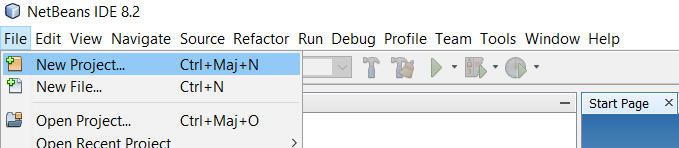
\includegraphics[width=\textwidth]{images/nb_newproject}
			\end{center}
		Nommez ce projet \texttt{td-java} et décochez la case \texttt{Create Main Class}.
			\begin{center}
				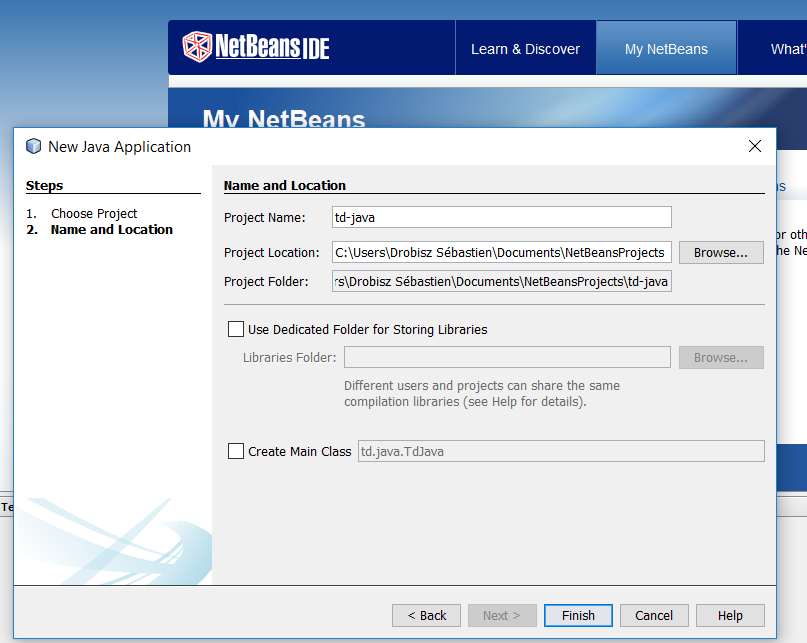
\includegraphics[width=\textwidth]{images/nb_newproject_name}
			\end{center}
			
		Dans Netbeans tout programme doit se trouver au sein d'un projet.
		Le projet contient le code de votre programme mais également les 
		information annexes comme le langage utilisé (ici Java), 
		la version du langage (ici nous utilisons Java 8), 
		et d'autres informations que vous découvrirez au fur et à mesure.

%		Un répertoire a été ajouté sur votre ordinateur. Trouvez le et vérifiez le contenu du dossier contenant les sources de votre projet. Le dossier sur votre ordinateur s'appelle \texttt{src}. S'il est vide, c'est normal, vous n'avez pas encore ajouté de source.


		\item Créez un package~: 
		
			Faites un clique droit sur le dossier contenant les sources de votre projet et 
			ajoutez un nouveau package Java.
		
			\bigskip
			\begin{center}
				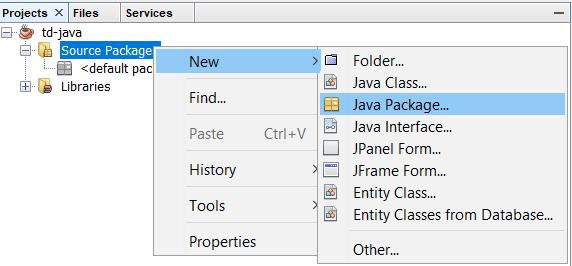
\includegraphics[width=\textwidth]{images/nb_newproject_package}
			\end{center}

			Nommez ce package \texttt{g12345.dev1.td1} où vous remplacez g12345 par votre identifiant~:
			\bigskip
			\begin{center}
				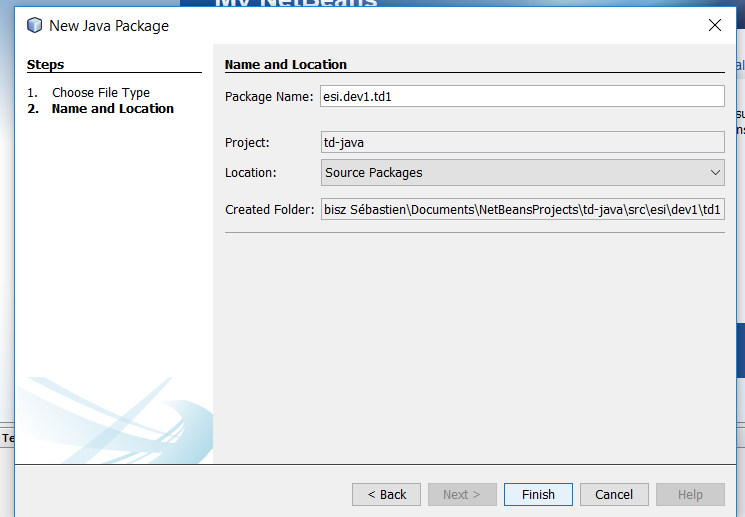
\includegraphics[width=\textwidth]{images/nb_newproject_package2}
			\end{center}
			
			En Java, un package (paquet) permet de regrouper certains morceaux de votre code
			et ainsi d'ordonner votre projet.

			Remarquez que ce package a été ajouté dans les sources de votre projet. 
			\bigskip
			\begin{center}
				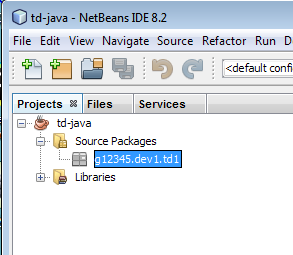
\includegraphics{images/nb_newproject_package3}
			\end{center}
%		Dans votre navigateur, vérifiez ce qui a été ajouté dans le dossier contenant vos sources.


		\item Créez une classe~:
		Dans NetBeans, faites un clique droit sur votre package 
		et ajoutez une nouvelle classe\footnote{Pour le moment, 
		on va simplement dire que c'est un fichier dans lequel se trouve du code Java.}. 
		Nommez cette classe {Hello}\footnote{Si vous oubliez la majuscule au H, 
		nous viendrons vous tirer les oreilles !}
		
		\bigskip
			\begin{center}
				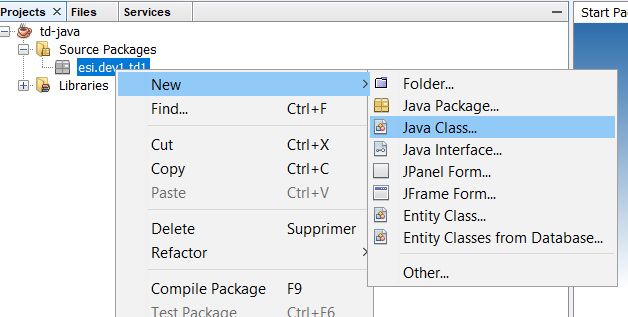
\includegraphics[width=\textwidth]{images/nb_newproject_new_class}
			\end{center}


		\item Cliquez sur votre classe \texttt{Hello}. Si vous voyez le code suivant, 
		veillez à l'effacer\footnote{Nous n'aimons pas le voir, il ne sert à rien}. 
			\begin{center}
				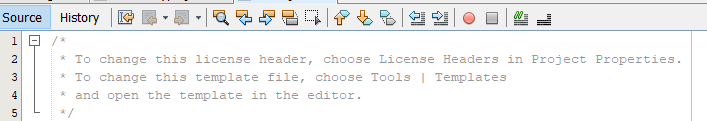
\includegraphics[width=\textwidth]{images/nb_newproject_header}
			\end{center}
			Faites la même chose pour le code contenant \texttt{/**...@author...*/}.
			Maintenant que c'est fait, ajoutez le code suivant :
	\begin{Code}{java}
	public static void main(String[] args) {
		System.out.println("Hello, World!");
	}
	\end{Code}
			Vous devriez obtenir ceci :
			\begin{center}
				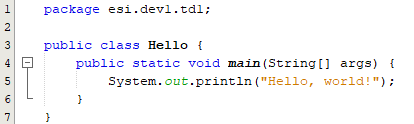
\includegraphics{images/nb_newproject_code}
			\end{center}
		\item Lancez le programme en cliquant sur la petite flèche \emph{run} 
		
\includegraphics{images/nb_newproject_run}.

		\item Modifiez votre programme pour que celui-ci affiche \texttt{"Hello"} suivi de votre prénom.

	\end{enumerate}


%===================
\section{Affichage}
%====================	

	% Exemple de rappel
	Le programme suivant affiche \texttt{Hello!} suivi de \texttt{Bonjour!}.
	\listing{Java}{code/HelloBonjour.java}

	En java l'affichage se fait par l'\emph{instruction}: \texttt{System.out.println("Hello!");}
	
	Le texte entre guillemets sera affiché sur la \emph{sortie standard}.

	% Fin du rappel
	%\hspeparator


	%Exercices
	\begin{Exercice}{Ligne}
		Dans votre package \texttt{g12345.dev1.td1} créez une classe \texttt{Ligne}.
		Dans cette classe écrivez un programme  (et donc dans la fonction \texttt{main} de cette classe) 
		qui affiche 10 tirets les uns à la suite des autres:

		\texttt{- - - - - - - - - -}
	\end{Exercice}
	
	\begin{Exercice}{Carré}
		Dans une classe \texttt{Carré}, écrivez un programme qui affiche un carré d'étoiles de 5 de côté:

		\begin{verbatim}
		*****
		*****
		*****
		*****
		*****
		\end{verbatim}
	\end{Exercice}

	\begin{Exercice}{Pyramide}
		Dans une classe \texttt{Pyramide}, écrivez un programme qui affiche une pyramide d'étoiles comme ceci:

		\begin{verbatim}
		   *
		  ***
		 *****
		*******
		\end{verbatim}
	\end{Exercice}

	\begin{Exercice}{Triangle}
		Dans une classe \texttt{Triangle}, écrivez un programme qui affiche un triangle d'étoiles comme ceci:

		\begin{verbatim}
		*
		**
		***
		****
		***
		**
		*
		\end{verbatim}
	\end{Exercice}




%===================
\section{Expressions}
%====================	

	Le programme suivant affiche la somme de 12345678 et 87654321.
	
	\listing{Java}{code/Expression.java}

	\begin{itemize}
		\item	L'instruction de la ligne 6 affiche le texte entre guillemets~: \texttt{12345678+87654321 = }
	
		\item L'instruction de la ligne 7 affiche le \emph{résultat du calcul} 
			c'est-à-dire la somme de 12345678 et de 87654321~:  \texttt{99999999}
	
		\item Notez que l'\emph{expresssion} \texttt{12345678+87654321} 
			de l'instruction de la ligne 7 ne se trouve \emph{pas} entre guillemets.
	\end{itemize}
	%\hspeparator


%% TODO: c'est exercices sont nuls, il faut les changer :-)
	\begin{Exercice}{}
		Dans une classe \texttt{Calculs}, écrivez un programme qui affiche la somme la valeur des expressions
		suivantes:
		\begin{itemize}
			\item	 \texttt{10 + 32}
			\item  \texttt{2 * 21}
			\item  \texttt{234\%57}
			\item  \texttt{((2*2)+(3*3))/25}
		\end{itemize}
	\end{Exercice}
	

%===================
\section{Variables}
%====================	

	Le programme suivant affiche l'aire d'un rectangle de longueur 12 et de largeur 4.
	
	\listing{Java}{code/Variables.java}

	\`A la ligne 6 la variable \texttt{longueur} est \emph{déclarée} avec le type \texttt{int}, 
	elle peut donc 'contenir' des entiers. 
	Sur cette même ligne on lui \emph{assigne} la valeur 12.  

	\`A la ligne 7 la variable \texttt{longueur} est \emph{déclarée} avec le type \texttt{int}. 
	Sur cette même ligne on lui \emph{assigne} la valeur 4.
	
	\`A la ligne 9 on affiche le résultat de la multiplication de la valeur de la variable \texttt{longueur}, 
	qui vaut 12, et de la valeur de la variable \texttt{largeur}, qui elle vaut 4.  
  



	\begin{Exercice}{} 		
		Dans un classe \texttt{VariablesExercice1} déclarez 2 variables~: 
		\texttt{x}, \texttt{y} et initialisez-les avec les valeurs 51 et 17.
		
		Ensuite affichez sur la sortie standard la valeur de :
		\begin{itemize}
		 	\item x+y
			\item x-y
			\item x*y
			\item x/y
			\item x\%y
			\item x*x+y*y
		\end{itemize} 
	\end{Exercice}

	\begin{Exercice}{} 
		Dans un classe \texttt{VariablesExercice2} déclarez 3 variables~: 
		\texttt{a}, \texttt{b} et \texttt{c} et initialisez avec les valeurs 2, 3 et 4 respectivement.
		
		Ensuite affichez sur la sortie standard la valeur de :
		\begin{itemize}
		 	\item 4 * a * c
			\item b*b - 4*a*c
		\end{itemize} 
	\end{Exercice}

%===================
\section{Lecture au clavier}
%====================	


	En java la lecture au clavier se fait en 3 étapes.

	\begin{enumerate}
		\item \emph{Importer} le \emph{lecteur} (\texttt{Scanner}) ligne 3 du code ci-dessous.
		\item \emph{Déclarer} et \emph{initialiser} le lecteur:  \texttt{Scanner clavier = new Scanner(System.in);}
		\item La lecture proprement dite: \texttt{int longueur = clavier.nextInt();}
	\end{enumerate}

	\listing{java}{code/AireRectangle.java}

	%\hspeparator


	\begin{Exercice}{Aire d'un carré}
		Dans une classe \texttt{AireRectangle}, écrivez un programme qui demande 
		le côté d'un carré à l'utilisateur et affiche l'aire de ce carré.
	\end{Exercice}

	\begin{Exercice}{} 
		Dans une classe \texttt{LectureExercice1}, écrivez un programme qui demande 
		deux nombres entiers, \texttt{x} et \texttt{y}, à l'utilisateur et afficher la valeur de :
		\begin{itemize}
		 	\item x+y
			\item x-y
			\item x*y
			\item x/y
			\item x*x+y*y
		\end{itemize} 
	\end{Exercice}


\section{Exercices}

	\begin{Exercice}{Aire d'un triangle }
		Dans une classe \texttt{AireTriangle}, écrivez un programme qui demande 
		la base et la hauteur d'un triangle rectangle à l'utilisateur et affiche son aire.
		
		Rappel: l'aire d'un triangle se calcule par la formule \texttt{(base*hauteur)/2}
		
	\end{Exercice}
	
	\begin{Exercice}{\texttt{HH:MM:SS} en secondes} 
		Dans une classe \texttt{Hms2s}, écrivez un programme qui demande 
		une nombre d'heures, un nombre de minutes et un nombre de secondes
		et qui affiche le nombre de secondes totales.
		
		Par exemple: si l'utilisateur entre 2 heures, 10 minutes et 27 secondes, le programme affiche
		7827. En effet 2 heures donnent 7200 secondes, 10 minutes sont 600 secondes 
		auxquelles il faut ajouter les 27 secondes: 7200 + 600 + 27 = 7827. 
	\end{Exercice}

	\begin{Exercice}{Secondes en minutes} 
	\end{Exercice}

	\begin{Exercice}{Secondes en heures} 
	\end{Exercice}


	\newpage
	\begin{Exercice}{Felix}
		Dans une classe \texttt{Felix}, écrivez un programme qui affiche le dessin suivant:

	\begin{verbatim}
	                          :                      :M
	                         XMX                   .HMM>
	                         MMMM.                dMMMM>
	                        'MMMMMX     .....   dMMMMMMX
	                        XMMMMMMMnMMMMMMMMMMMMMMMMMMM
	                       :MMMMMMMMMMMMMMMMMMMMMMMMMMMM>
	                       XMMMMM!"    "MMMMMM"`  `"MMMMM
	                       MMMM#         4MMf        `MMMX
	                      XMMM            MX          'MMM:
	                     'MMM~            '>            MMM
	                     MMMf       .     '>            `MMX
	                    MMMM>     :MMM    '>   :MMM      MMMX
	                   XMMMM      MMMM>   '>   XMMMX     MMMMk
	                  MMMMMM>     MMMM~   'k   MMMMX     MMMMMh
	                 MMMMMMMX     XMMM    XX   ?MMM     XMMMMMMM
	                 MMMMMMMMk     ^`    X 'h    `     :MM##MMM~
	                  ?MM>  ^?M.       .!    %.      .HM"   MM
	                 .?M      '"%+++!".nMMMMn "%++!*" %.. 'M..
	                  `?M>+%L         <MMMMMMMM>       :   XM"
	                    'X   %        XMMMMMMMM>      X   'f
	                      X   `M.      ?MMMMMM~    .HM   :`
	                       %.  `MMMx.          .xHMMM   X
	                  ..    `X  `MMMMMMMMMMMMMMMMMMM  :f
	                :MMMMMMMh:.M. 4MM     "     MM" xMMMMMMMMMMh.
	              :MMMMMMMMMMMMMMM: `%x.......x"`.HMMMMMMMMMMMMMM
	            .MMMMMMMMMMMMMMMMMMMMhx.......xHMMMMMMMMMMMMMMMMM
	    .nHMMMMMMMMMMMMMMMMMMMMMMMMMMMMMMMMMMMM`MMMMMMMMMMMMMMMMX
	  :MMMMMMMMMMMMMMMMMMMMMMMMMMMMMMMMMMMMdMMMMMMMMMMMMMMMMMMMM
	 MMMMMMMMMMMMMMMMMMMM"``""MMMMMMMMMMMM!MMMMMMMMMMMMMMMMMMMM~
	MMMMMMMMMMMMMMMMMMM!     XMMMMMMMMMMMf:HMMMMMMMMMMMMMMMMM!
	M?MMMMMMMMMMMMMMMM`    :MMMMMMMMMMMM!MMMMMMMMMMMMMMMMMMM~
	:MMMMMMMMMMMMMMMMX     MMMMMMMMMMMMXXMMMMMMMMMMMMMMMMM`
	MMMMMMMMMMMMMMMMMX    'MMMMMMMMMMMMM!MMMMMMMMMMMMMMMMX
	MMMMMMMMMMMMMMMMM~    'MMMMMMMMMMMMMM?MMMMMMMMMMMMMMM~
	 #M)MMMMMMMM!MMM       MMMMMMMMMMMMMMMM/MMMMMMMMMMMM~
	   ?MMMMMM"-"2MMMMMx   XMMMMMMMMMMMMMMMMX?**!:MMM"`
	\end{verbatim}
\end{Exercice}




\end{document}